%% ============================================================================
\section{Lecture 9: The Convective Phase Space, Shear, and the Equipartition Principle}
\label{sec:lec09}
%% ============================================================================
\date{11/06/2026}

\begin{center}
    \textit{Lecture date: 11/06/2026}
\end{center}

This lecture completes the dimensional-analysis description of thermal
convection begun in Lectures~7--8 and then opens a new estimation theme. In the
first half we finish counting the dimensionless groups of the
Rayleigh--B\'enard problem: beyond the Prandtl and Rayleigh numbers we identify
the Boussinesq parameter $\alpha\Delta T$ and a gravitational-compressibility
parameter $\alpha gH/c_p$, show that both are tiny under laboratory conditions,
and conclude that ordinary convection lives in a \emph{two-dimensional} phase
space $(\mathrm{Ra},\mathrm{Pr})$. We then extract the typical convective
velocity, ask how an externally imposed shear competes with convection
(Richardson number), and how fast convection can ever become (Mach number).

In the second half we introduce the \emph{equipartition principle} as a general
estimation strategy: in a coupled system, energy tends to distribute itself
comparably among the interacting components --- exactly so for quadratic
energies, and up to factors of order unity otherwise. We use it to estimate the
Bohr radius, the ground state of an anharmonic potential, the frequency of an
LC circuit, and the energy content of the interstellar medium, and we derive
hydrostatic equilibrium and the Euler equation as the setup for next week's
estimate of the Chandrasekhar mass.


%%----------------------------------------------------------------------------
\subsection{Recap: The Dimensionless Groups of Rayleigh--B\'enard Convection}
\label{sec:lec09:recap}
%%----------------------------------------------------------------------------

\subsubsection*{Mathematical Setup}
A fluid layer heated from below is described by eight dimensional quantities:
the layer height $H$, the imposed temperature difference $\Delta T$, the
density $\rho$, the kinematic viscosity (momentum diffusivity) $\nu$, the
thermal diffusivity $\chi$, the gravitational acceleration $g$, the thermal
expansion coefficient $\alpha$ defined through
\begin{equation}
    \rho=\rho_0\left(1-\alpha\Delta T\right),
    \label{eq:lec09:expansion-law}
\end{equation}
and the specific heat capacity $c_p$. These involve four independent
dimensions (mass, length, time, temperature), so by the Buckingham
$\Pi$ theorem the problem is governed by $8-4=4$ dimensionless groups.

Two of the groups were constructed in Lecture~8:
\begin{equation}
    \Pi_1=\mathrm{Pr}\equiv\frac{\nu}{\chi},
    \qquad
    \Pi_2=\mathrm{Gr}\equiv\frac{g\alpha\Delta T\,H^3}{\nu^2}.
    \label{eq:lec09:pr-gr}
\end{equation}
The Prandtl number is a \emph{material} property: it compares how easily the
fluid diffuses momentum versus heat. The Grashof number is the square of the
Reynolds number of the flow,
\begin{equation}
    \mathrm{Gr}=\left(\frac{UH}{\nu}\right)^2=\mathrm{Re}^2,
    \qquad
    U^2\sim g\alpha\Delta T\,H,
    \label{eq:lec09:gr-re}
\end{equation}
but computed with the velocity that the system \emph{generates by itself}
through buoyancy (a hot element of fractional density deficit
$\alpha\Delta T$ accelerates at $g\alpha\Delta T$ over the scale $H$), not
with an externally imposed velocity.

In practice one works with the Rayleigh number
\begin{equation}
    \mathrm{Ra}\equiv\mathrm{Gr}\,\mathrm{Pr}
    =\frac{g\alpha\Delta T\,H^3}{\nu\chi},
    \label{eq:lec09:rayleigh}
\end{equation}
because the criterion for the onset of convection is expressed through it:
even a superadiabatic gradient does not guarantee convection, since the system
may prefer to transport the heat diffusively. Linear stability analysis of a
closed layer gives
\begin{equation}
    \boxed{
    \text{convection sets in}
    \iff
    \mathrm{Ra}>\mathrm{Ra}_c,
    \qquad
    \mathrm{Ra}_c\simeq
    \begin{cases}
        \sim 1100 & \text{free upper surface (open pot)},\\[2pt]
        \sim 1700 & \text{rigid--rigid boundaries}.
    \end{cases}
    }
    \label{eq:lec09:critical-rayleigh}
\end{equation}
\textit{Significance:} The onset of convection is not a local property of the
temperature gradient alone; it is a global competition between buoyant driving
($g\alpha\Delta T H^3$) and the two dissipative diffusivities ($\nu\chi$), and
it depends on the boundary conditions.

\nt{The critical values and the full classification of boundary conditions
(including added magnetic fields) are worked out in S.~Chandrasekhar's
classic monograph \emph{Hydrodynamic and Hydromagnetic Stability}.
Chandrasekhar received the Nobel Prize for his work on white dwarfs --- the
very topic this lecture turns to at the end.}

%%----------------------------------------------------------------------------
\subsection{The Third Group: The Boussinesq Parameter \texorpdfstring{$\alpha\Delta T$}{alpha dT}}
\label{sec:lec09:boussinesq}
%%----------------------------------------------------------------------------

\subsubsection*{Physical Motivation}
The combination $\alpha\Delta T$ is already dimensionless, so it is a
legitimate third group:
\begin{equation}
    \Pi_3\equiv\alpha\Delta T.
    \label{eq:lec09:pi3-definition}
\end{equation}
What does it measure? Two equivalent readings:
\begin{itemize}
    \item \textbf{Density contrast.} By Eq.~\eqref{eq:lec09:expansion-law},
    $\alpha\Delta T=\abs{\Delta\rho}/\rho_0$ is the fractional density change
    across the layer.
    \item \textbf{Acceleration relative to gravity.} The buoyant acceleration
    of a hot element is $a_{\rm buoy}=g\alpha\Delta T$ (Archimedes), so
    \begin{equation}
        \boxed{
        \Pi_3=\alpha\Delta T
        =\frac{\abs{\Delta\rho}}{\rho_0}
        =\frac{a_{\rm buoy}}{g}.
        }
        \label{eq:lec09:pi3-meaning}
    \end{equation}
\end{itemize}
\textit{Significance:} A buoyant element can never accelerate faster than $g$
itself; $\Pi_3$ tells us how far the system is from that saturation, i.e.\ how
strongly nonlinear the convection is.

\subsubsection*{Validity Regime}
\begin{itemize}
    \item If $\alpha\Delta T\ll 1$ the problem is \emph{linear in the
    forcing}: doubling $\Delta T$ simply doubles all density perturbations and
    accelerations without changing the character of the solution. This is the
    Boussinesq regime in which the expansion
    \eqref{eq:lec09:expansion-law} is justified.
    \item Once $\alpha\Delta T=\order{1}$ the linearization of $\rho(T)$
    breaks down, the truncated expansion is no longer a valid equation of
    state, and the behaviour can change qualitatively --- new powers, new
    prefactors, possibly no simple scaling solution at all.
\end{itemize}

\nt{Pitfall: $\Delta T$ here can be defined either locally (between two
adjacent elements) or globally (between the bottom and the top of the entire
system). Locally $\alpha\Delta T$ is essentially always small; globally it can
be large, in which case $\rho=\rho_0(1-\alpha\Delta T)$ written with
$\rho_0$ the bottom density is simply not a valid description, and a
nonlinear equation of state must be used. Always state which $\Delta T$ a
dimensionless number is built from.}

%%----------------------------------------------------------------------------
\subsection{The Fourth Group: Thermal versus Gravitational Energy}
\label{sec:lec09:fourth-group}
%%----------------------------------------------------------------------------

\subsubsection*{Physical Motivation}
We want one more group, and we want it to compare a length scale that
characterizes the \emph{fluid} (not the container) to the system size $H$. The
heat capacity $c_p$ has not yet been used independently, so the new group must
contain it. The physical question that isolates $c_p$ is: convection
transports \emph{internal thermal} energy, $c_p\Delta T$ per unit mass; but
the moving elements also exchange \emph{gravitational} energy. Over what
distance does the gravitational energy become comparable to the thermal energy
being carried?

\subsubsection*{Derivation}
Take an element with temperature excess $\Delta T$:
\begin{itemize}
    \item Thermal energy carried per unit mass: $c_p\Delta T$.
    \item Buoyancy force per unit mass: $a_{\rm buoy}=g\alpha\Delta T$.
    \item Mechanical (gravitational) energy per unit mass gained over a
    distance $\lambda$: force per unit mass times distance,
    $g\alpha\Delta T\,\lambda$.
\end{itemize}
Demanding that the two energies be comparable,
\begin{equation}
    g\alpha\Delta T\,\lambda\sim c_p\Delta T
    \quad\Longrightarrow\quad
    \frac{g\alpha\lambda}{c_p}\sim 1,
    \label{eq:lec09:lambda-balance}
\end{equation}
defines an intrinsic length scale of the fluid (note that $\Delta T$ cancels):
\begin{equation}
    \boxed{
    \lambda\equiv\frac{c_p}{\alpha g}.
    }
    \label{eq:lec09:lambda-definition}
\end{equation}
\textit{Significance:} $\lambda$ is the distance over which the gravitational
potential energy of a convecting element becomes comparable to the thermal
energy it carries; below this scale gravity's energetic bookkeeping is
negligible and only buoyancy's \emph{force} matters.

The fourth dimensionless group is then
\begin{equation}
    \boxed{
    \Pi_4\equiv\frac{H}{\lambda}=\frac{\alpha gH}{c_p}.
    }
    \label{eq:lec09:pi4-definition}
\end{equation}

\ex{Worked Example: Is Gravity Energetically Relevant in a Pot of Water?}{
For water on Earth, $c_p\simeq 4.2\times10^{3}\,\si{J.kg^{-1}.K^{-1}}$ and
$\alpha g\sim\order{10^{-3}}\,\si{m.s^{-2}.K^{-1}}$, giving
\[
    \lambda=\frac{c_p}{\alpha g}\sim\text{a few}\times 10^{2}\,\si{km}
    \qquad(\text{the value quoted in class: }\sim 200\,\si{km}).
\]
A $30\,\si{cm}$ pot, and even a few-km-deep ocean, has $H\ll\lambda$, so
$\Pi_4\ll1$: the gravitational potential energy of the convecting elements is
irrelevant and may be dropped from the model. Only for a hypothetical
planetary-scale ocean with $H\gtrsim10^{3}\,\si{km}$ would $\Pi_4$ approach
unity --- and then a laboratory experiment could \emph{not} be scaled up to the
planet, because the large system contains physics (gravitational energetics,
compressibility) that the small one does not.
}

\nt{Connection to Lectures 7--8: for an ideal gas $\alpha=1/T$, so
$\lambda=c_pT/g$, which is exactly the depth over which adiabatic
compression changes the temperature by $\order{T}$ --- the inverse of the
adiabatic gradient $\Gamma_{\rm ad}=g/c_p$. Thus $\Pi_4=H/\lambda$ is the
compressibility parameter that decides whether one must distinguish
$\Gamma$ from $\Gamma-\Gamma_{\rm ad}$. In a shallow pot $\Pi_4\ll1$ and the
adiabatic correction is negligible; in an atmosphere or a star $\Pi_4\gtrsim1$
and it is essential.}

\subsubsection*{Method: Constructing Additional Dimensionless Groups}
After $k$ groups have been found, infinitely many further combinations exist
(any product of powers of the existing ones); the lecturer's recipe for
choosing a \emph{useful} new group:
\begin{enumerate}
    \item It must contain a variable not yet used independently (here $c_p$)
    --- otherwise it is a combination of the known groups (linear algebra in
    the exponent space).
    \item Prefer groups that are purely material properties (like
    $\mathrm{Pr}$), or purely ratios of system scales, avoiding $\Delta T$ and
    $H$ when possible --- such groups are reusable across systems.
    \item Give the group a physical reading by equating two \emph{energies} or
    two \emph{rates} of competing physical processes. It is legitimate to
    introduce a temporary auxiliary quantity (here $\lambda$) to make the
    meaning transparent --- this does not add a ninth parameter, it is defined
    by the others.
    \item Any pair of physical processes can be compared this way: convective
    versus conductive heat transport, convective transport versus radiative
    losses, etc. In massive stars, convection near the surface is quenched
    because a rising element \emph{radiates} its heat away faster than it
    rises --- a new dimensionless ratio signals new physics.
\end{enumerate}

\nt{Homework pointer: the current problem set asks to estimate the heat
transported by convection versus by conduction (their ratio is the Nusselt
number of Lecture~8, expressible through the groups found here), and to
estimate the radiative loss of the same system --- precisely steps 3--4 of
this recipe.}

%%----------------------------------------------------------------------------
\subsection{The Two-Dimensional Phase Space of Laboratory Convection}
\label{sec:lec09:phase-space}
%%----------------------------------------------------------------------------

\subsubsection*{Conceptual Background}
For everyday systems (a soup pot, a laboratory cell) both $\Pi_3=\alpha\Delta
T$ and $\Pi_4=\alpha gH/c_p$ are tiny. The four-dimensional parameter space
therefore collapses: \emph{the state of the convection is characterized by two
numbers only}, $(\mathrm{Ra},\mathrm{Pr})$ --- or equivalently
$(\mathrm{Gr},\mathrm{Pr})$ --- once the geometry and boundary conditions are
fixed.

\begin{figure}[ht]
    \centering
    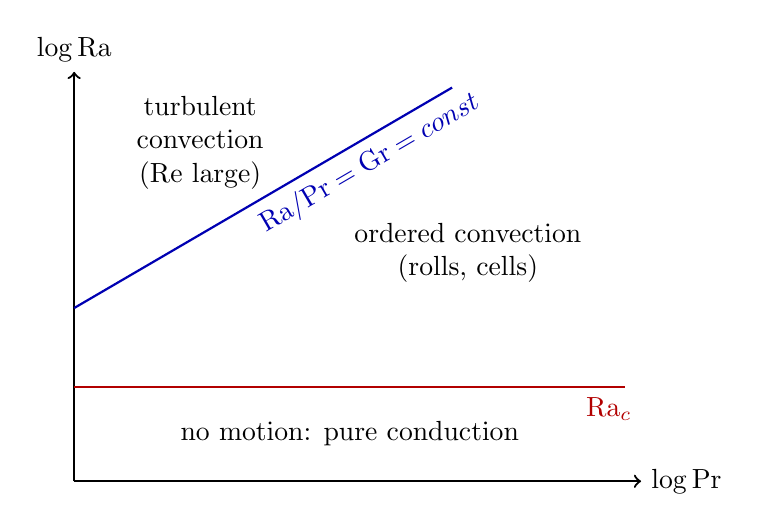
\begin{tikzpicture}[scale=1.0]
        % axes (log-log)
        \draw[thick,->] (0,0) -- (7.2,0) node[right] {$\log\mathrm{Pr}$};
        \draw[thick,->] (0,0) -- (0,5.2) node[above] {$\log\mathrm{Ra}$};
        % critical Rayleigh line
        \draw[thick,red!70!black] (0,1.2) -- (7,1.2)
            node[pos=0.97,below] {$\mathrm{Ra}_c$};
        \node[align=center] at (3.5,0.6)
            {no motion: pure conduction};
        % constant-Gr (slope 1) line separating turbulent / ordered
        \draw[thick,blue!70!black] (0.0,2.2) -- (4.8,5.0)
            node[pos=0.75,below,sloped] {$\mathrm{Ra}/\mathrm{Pr}=\mathrm{Gr}=\text{const}$};
        \node[align=center] at (1.6,4.3)
            {turbulent\\convection\\($\mathrm{Re}$ large)};
        \node[align=center] at (5.0,2.9)
            {ordered convection\\(rolls, cells)};
    \end{tikzpicture}
    \caption{Schematic phase diagram of Rayleigh--B\'enard convection in the
    $(\mathrm{Pr},\mathrm{Ra})$ plane. Below $\mathrm{Ra}_c$ heat is carried
    by conduction only. Above it, the character of the flow is set by the
    effective Reynolds number $\mathrm{Re}=\sqrt{\mathrm{Ra}/\mathrm{Pr}}$:
    lines of constant $\mathrm{Gr}=\mathrm{Re}^2$ have slope $1$ in the
    log--log plane, separating ordered rolls (low $\mathrm{Re}$) from
    turbulence (high $\mathrm{Re}$).}
    \label{fig:lec09:phase-diagram}
\end{figure}

\subsubsection*{Reading the Diagram}
Since $\mathrm{Gr}=\mathrm{Ra}/\mathrm{Pr}=\mathrm{Re}^2$ is the squared
Reynolds number of the self-generated flow:
\begin{itemize}
    \item $\mathrm{Ra}<\mathrm{Ra}_c$: no motion at all; the layer conducts.
    \item $\mathrm{Ra}>\mathrm{Ra}_c$ with moderate
    $\mathrm{Re}=\sqrt{\mathrm{Ra}/\mathrm{Pr}}$: \emph{ordered} convection
    --- beautiful rolls or polygonal cells.
    \item $\mathrm{Ra}>\mathrm{Ra}_c$ with large $\mathrm{Re}$:
    \emph{turbulent} convection.
\end{itemize}
Experimentally one scans this plane by varying the heating
($\mathrm{Ra}\propto\Delta T$) and by switching fluids: dissolving honey in
water raises $\nu$ without much changing $\chi$, raising $\mathrm{Pr}$ at
will. Classic experimental sequences (shown in class) sample
$\mathrm{Ra}/\mathrm{Ra}_c-1$ from just above $0$ up to tens, at
$\mathrm{Pr}=\order{1}$, and watch the rolls appear and then disorder.

\nt{Kitchen-physics aside: thickening soup with cornflour raises
$\mathrm{Pr}$ strongly (long starch chains give high viscosity but poor heat
conduction), which is why slow ordered convection rolls are visible in thick
orange soup. Cornflour suspensions are also non-Newtonian
(shear-thickening): the viscosity itself grows with the velocity gradient, so
a single $\mathrm{Pr}$ no longer characterizes the fluid.}

%%----------------------------------------------------------------------------
\subsection{The Typical Convective Velocity and \texorpdfstring{$\Pi_5$}{Pi5}}
\label{sec:lec09:typical-velocity}
%%----------------------------------------------------------------------------

\subsubsection*{Derivation}
What velocity does the convection develop? Build the simplest possible model:
the element undergoes free fall under the \emph{effective} gravity
$g_{\rm eff}=g\alpha\Delta T$ over the distance $H$. For free fall,
$v^2=2g_{\rm eff}H$, so up to the factor of $2$,
\begin{equation}
    \boxed{
    V_T^2\equiv g\alpha\Delta T\,H.
    }
    \label{eq:lec09:vtypical}
\end{equation}
\textit{Significance:} This is the same buoyancy-velocity estimate as
Lecture~8, now promoted to the \emph{unit} in which the true velocity is
measured.

The actual velocity in the cell defines a fifth (dependent) dimensionless
number,
\begin{equation}
    \Pi_5\equiv\frac{V_{\rm actual}}{V_T},
    \label{eq:lec09:pi5-definition}
\end{equation}
and dimensional analysis guarantees a functional relation
$\tilde F(\Pi_5,\mathrm{Ra},\mathrm{Pr})=0$, which can be inverted to
\begin{equation}
    \boxed{
    V_{\rm actual}^2
    =
    g\alpha\Delta T\,H\;
    f\!\left(\mathrm{Ra},\mathrm{Pr}\right).
    }
    \label{eq:lec09:velocity-scaling}
\end{equation}
\textit{Significance:} Dimensional analysis fixes everything except the
order-unity function $f$ of the two governing groups; $f$ is then measured
once and for all in the laboratory or in a simulation, for every point of the
two-dimensional phase space. If the system is planetary-scale, $\Pi_4$ can no
longer be dropped and the parameter space becomes three-dimensional ---
unless one restricts attention to a fixed fluid (e.g.\ water,
$\mathrm{Pr}=\order{1}$), which removes one axis again.

%%----------------------------------------------------------------------------
\subsection{External Shear: The Richardson Number}
\label{sec:lec09:richardson}
%%----------------------------------------------------------------------------

\subsubsection*{Physical Motivation}
Now complicate the problem: impose an external \emph{shear} --- a velocity that
varies with height, $\dd V_{\rm ext}/\dd z\neq0$ (stirring the pot, or wind
speed changing with altitude). Strong shear tears apart the coherent rising
and sinking elements, so it can destroy convection. Which dimensionless number
decides?

\subsubsection*{Derivation}
The convection itself possesses an \emph{internal} shear: the buoyancy
velocity $V_T$ develops over the scale $H$, so
\begin{equation}
    \left(\dv{V}{z}\right)_{\rm int}
    \sim\frac{V_T}{H}
    =\frac{\sqrt{g\alpha\Delta T\,H}}{H}
    =\sqrt{\frac{g\alpha\Delta T}{H}}.
    \label{eq:lec09:internal-shear}
\end{equation}
The externally imposed shear is
\begin{equation}
    \left(\dv{V}{z}\right)_{\rm ext}
    \sim\frac{\Delta V_{\rm ext}}{H},
    \label{eq:lec09:external-shear}
\end{equation}
where $\Delta V_{\rm ext}$ is the velocity difference between the bottom and
the top. The Richardson number is defined as the squared ratio (squared
historically, to dispose of the square root):
\begin{align}
    \mathrm{Ri}
    &\equiv
    \frac{\left(\dd V/\dd z\right)_{\rm int}^2}
         {\left(\dd V/\dd z\right)_{\rm ext}^2}
    =
    \frac{g\alpha\Delta T/H}{\Delta V_{\rm ext}^2/H^2},
    \label{eq:lec09:richardson-step}
\end{align}
so
\begin{equation}
    \boxed{
    \mathrm{Ri}
    =
    \frac{g\alpha\Delta T\,H}{\Delta V_{\rm ext}^2}
    =
    \frac{V_T^2}{\Delta V_{\rm ext}^2}.
    }
    \label{eq:lec09:richardson}
\end{equation}
\textit{Significance:} $\mathrm{Ri}$ compares the buoyant kinetic energy the
convection generates to the kinetic energy of the imposed shear; it decides
whether convection survives an external velocity gradient.

\nt{Pitfall: the Richardson convention is \emph{inverted} relative to the
physicists' habit of ``small parameter $=$ unimportant process''. Here
$\mathrm{Ri}\gg1$ means the shear is \emph{unimportant} (internal motions
dominate), while $\mathrm{Ri}\lesssim1$ means the shear \emph{matters}.
Several variants exist, differing by which velocity derivative is taken
(vertical wind shear, horizontal shear from stirring, etc.) --- check the
definition before quoting thresholds.}

\subsubsection*{Validity Regimes and Atmospheric Consequences}
\begin{itemize}
    \item $\mathrm{Ri}\lesssim1$: the shear is energetically dominant. It
    destroys buoyant convection and itself drives turbulence
    (shear/Kelvin--Helmholtz instability) \emph{regardless} of whether the
    stratification is convectively unstable. The wavy billows seen in high
    clouds at jet-stream altitude are exactly this instability.
    \item Intermediate $\mathrm{Ri}$: shear and buoyancy cooperate; the shear
    organizes the convection into a single long-lived rotating updraft --- a
    \emph{supercell} (the parent of large cumulonimbus storms).
    \item $\mathrm{Ri}\gtrsim40$ (meteorological threshold quoted in class):
    the shear is negligible; convection breaks into many small short-lived
    cells (\emph{multicell} convection), and no large supercells form.
\end{itemize}

\nt{Remark on turbulent cascades (class discussion): three-dimensional
turbulence cascades energy from large eddies to small ones, where viscosity
dissipates it. Two-dimensional (or strongly stratified, layered) turbulence
behaves oppositely: an additional conserved quantity forces an \emph{inverse
cascade}, and vortices merge into ever larger ones. This is why thin layered
flows --- e.g.\ where a fresh river current slides over salty sea water, as at
the St.~Lawrence estuary --- show long-lived coherent vortices that grow by
pairwise merging instead of decaying.}

%%----------------------------------------------------------------------------
\subsection{How Fast Can Convection Get? The Mach Number}
\label{sec:lec09:mach}
%%----------------------------------------------------------------------------

\subsubsection*{Physical Motivation}
One more physically meaningful comparison is available: the convective
velocity versus the sound speed,
\begin{equation}
    c_s\sim\sqrt{\frac{k_BT}{\bar m}},
    \label{eq:lec09:sound-speed}
\end{equation}
with $\bar m$ the mean molecular mass. This introduces compressibility ---
new physics --- and with it a sixth group:
\begin{equation}
    \boxed{
    \Pi_6\equiv\frac{V}{c_s}=\mathcal{M}
    \qquad\text{(Mach number)}.
    }
    \label{eq:lec09:mach}
\end{equation}
\textit{Significance:} When convection approaches $\mathcal{M}\sim1$, shock
waves form; shocks dissipate the kinetic energy of the flow and thereby
\emph{cap} the convective velocity. Sonic convection,
$V\sim c_s$, is therefore the most efficient convection achievable --- a limit
of central importance in astrophysics (stellar envelopes), where buoyant
driving can be enormous.

%%----------------------------------------------------------------------------
\subsection{The Equipartition Principle as an Estimation Tool}
\label{sec:lec09:equipartition}
%%----------------------------------------------------------------------------

\subsubsection*{Conceptual Background}
We met the idea of comparing energies at the very start of the course; now we
elevate it to a systematic estimation principle.

\clm[clm:lec09:equipartition]{Equipartition Estimation Principle}{
In a system whose components exchange energy through some coupling process,
the energy (or energy density) of each component is driven toward the same
order of magnitude. When all the energies are \emph{quadratic} in their basic
variable (harmonic oscillator, LC circuit, acoustic wave), the time-averaged
equality is exact; for other power laws it holds up to a dimensionless factor
of order unity.
}

The exact backing is the virial theorem: for a bound particle in a power-law
potential $V(x)=\alpha\abs{x}^{\,n}$,
\begin{equation}
    \boxed{
    2\expval{T}=n\expval{V},
    }
    \label{eq:lec09:virial}
\end{equation}
so $\expval{T}=\expval{V}$ exactly for the harmonic case $n=2$,
$\expval{T}=-\tfrac12\expval{V}$ for gravity/Coulomb ($n=-1$), and
$\expval{T}=\tfrac32\expval{V}$ for $n=3$ --- always the same order of
magnitude. The estimation strategy is therefore: \emph{identify the two (or
more) energy reservoirs, equate them, and solve for the unknown}.

\subsubsection*{Physical Motivation: Equipartition in the Interstellar Medium}
A striking large-scale example: in the interstellar medium (ISM) the energy
densities of four entirely different components are all comparable,
\begin{equation}
    u_{\rm th}\sim n\,\tfrac32 k_BT,
    \quad
    u_{B}=\frac{B^2}{8\pi},
    \quad
    u_{\rm CR}\sim n_{\rm CR}\expval{E_{\rm CR}},
    \quad
    u_{\rm turb}\sim\tfrac12\rho\expval{v^2},
    \label{eq:lec09:ism-components}
\end{equation}
and each is of order
\begin{equation}
    \boxed{
    u_{\rm ISM}\sim1\,\si{eV.cm^{-3}}
    }
    \label{eq:lec09:ism-energy-density}
\end{equation}
up to factors of a few.
\textit{Significance:} This is not numerology --- concrete processes couple
the reservoirs and saturate precisely when the energy densities match.

Why the coupling works:
\begin{itemize}
    \item \textbf{Magnetic field $\leftrightarrow$ turbulence:} in a
    conducting plasma the field is \emph{frozen} into the matter (flux
    freezing); moving gas clouds stretch the field lines like rubber bands.
    The stretching continues until the magnetic stress is strong enough to
    resist the turbulent motion --- i.e.\ until $u_B\sim u_{\rm turb}$.
    \item \textbf{Cosmic rays $\leftrightarrow$ the rest:} cosmic-ray
    acceleration draws on the same energy reservoirs and saturates when the
    cosmic-ray energy density becomes comparable to that of the accelerating
    agent.
    \item \textbf{Timescales:} equilibration requires the coupling time to be
    much shorter than the system's age. Here the timescales are
    $\lesssim10^{6\text{--}7}$ years --- e.g.\ the cosmic-ray residence age is
    measured to be $\sim10^{7}\,\mathrm{yr}$ from the isotope ratio of
    $^{10}$Be (half-life $\sim10^{6}\,\mathrm{yr}$) to stable beryllium ---
    far shorter than the Galaxy's age, so equipartition has had time to
    establish itself.
\end{itemize}

\ex[ex:lec09:bohr-radius]{Worked Example: The Bohr Radius from Energy Balance}{
Estimate the size of the hydrogen atom \emph{without} dimensional analysis
(done in a previous lecture), by comparing energies.

\textbf{Potential energy} at radius $a_0$ (Gaussian units):
\[
    \abs{E_{\rm pot}}\sim\frac{e^2}{a_0}.
\]
\textbf{Kinetic energy}: confining the electron to a region of size $a_0$
costs momentum by the uncertainty principle, $p\sim\hbar/a_0$, hence
\[
    E_{\rm kin}\sim\frac{p^2}{2m_e}=\frac{\hbar^2}{2m_e a_0^2}.
\]
This is the essential quantum input: squeezing the electron into a smaller
radius \emph{raises} its kinetic energy, which is what halts the collapse.
The ground state sits where the two energies are comparable:
\[
    \frac{e^2}{a_0}\sim\frac{\hbar^2}{2m_e a_0^2}
    \quad\Longrightarrow\quad
    \boxed{
    a_0\sim\frac{\hbar^2}{m_e e^2}
    }
\]
(the factor $2$ is meaningless at this accuracy and is dropped). The exact
Bohr radius is $\hbar^2/m_ee^2$ --- the order-unity factor happens to be $1$.
}

\ex[ex:lec09:cubic-well]{Worked Example: Ground State of $V(x)=\alpha\abs{x}^3$
(exam-style)}{
Find the ground-state energy of a particle of mass $m$ in the anharmonic well
$V(x)=\alpha\abs{x}^{3}$ --- a potential with no exact closed-form solution.

\textbf{Step 1 — kinetic energy of confinement.} If the wavefunction has
spread $\Delta x$, then $\Delta p\sim\hbar/\Delta x$ and
\[
    E_{\rm kin}\sim\frac{\hbar^2}{2m\,\Delta x^2}.
\]
\textbf{Step 2 — potential energy at that spread:}
\[
    E_{\rm pot}\sim\alpha\,\Delta x^{3}.
\]
\textbf{Step 3 — equipartition:} the ground state balances the two,
\[
    \alpha\,\Delta x^{3}\sim\frac{\hbar^2}{2m\,\Delta x^{2}}
    \quad\Longrightarrow\quad
    \Delta x^{5}\sim\frac{\hbar^{2}}{2m\alpha}
    \quad\Longrightarrow\quad
    \Delta x\sim\left(\frac{\hbar^{2}}{2m\alpha}\right)^{1/5}.
\]
\textbf{Step 4 — evaluate either energy at $\Delta x$} (they are equal by
construction, so either one gives the answer up to a unit factor):
\[
    \boxed{
    E_{0}\sim\alpha\,\Delta x^{3}
    =\alpha\left(\frac{\hbar^{2}}{2m\alpha}\right)^{3/5}
    =\alpha^{2/5}\left(\frac{\hbar^{2}}{2m}\right)^{3/5}.
    }
\]
The unknown prefactor is a pure number of order unity, fixed only by actually
solving the Schr\"odinger equation.
}

\cor[cor:lec09:powerlaw-ground-state]{Ground State of a General Power-Law Well}{
The same three steps for $V(x)=\alpha\abs{x}^{\,n}$ ($n>0$) give
\[
    \Delta x\sim\left(\frac{\hbar^{2}}{2m\alpha}\right)^{\frac{1}{n+2}},
    \qquad
    E_{0}\sim\alpha^{\frac{2}{n+2}}
    \left(\frac{\hbar^{2}}{2m}\right)^{\frac{n}{n+2}}.
\]
Check: $n=2$ with $\alpha=\tfrac12 m\omega^2$ reproduces
$E_0\sim\hbar\omega$, as it must.
}

\subsubsection*{Method: Quantum Ground-State Estimates}
\begin{enumerate}
    \item Write the potential energy at the unknown spread,
    $E_{\rm pot}=V(\Delta x)$.
    \item Write the confinement kinetic energy
    $E_{\rm kin}=\hbar^2/2m\Delta x^2$ from
    $\Delta p\sim\hbar/\Delta x$.
    \item Set $E_{\rm pot}\sim E_{\rm kin}$ and solve for $\Delta x$.
    \item Substitute back into either energy --- that is $E_0$ up to an
    order-unity factor.
\end{enumerate}

\nt{Pitfall: do not carry the spurious factor of $2$ (or any other unit
factor) through such an estimate as though it were significant --- the method
is blind to order-unity numbers, and quoting $\hbar^2/2me^2$ rather than
$\hbar^2/me^2$ for the Bohr radius conveys false precision. Also note the
estimate gives the \emph{ground} level; for highly excited levels the same
balance with $\Delta x\,\Delta p\sim n\hbar$ gives the scale of the $n$-th
level and of the level \emph{spacing}, but the accuracy in the absolute energy
degrades since the order-unity ignorance multiplies a larger number.}

\ex[ex:lec09:lc-circuit]{Worked Example: Frequency of an LC Circuit}{
An inductor $L$ and capacitor $C$ exchange energy periodically. The two
reservoirs are
\[
    E_C=\frac{Q^2}{2C},
    \qquad
    E_L=\frac{LI^2}{2}.
\]
Both are quadratic in their basic variables, so the system is harmonic and
equipartition is \emph{exact} on average: $\expval{E_C}=\expval{E_L}$. For an
oscillation at frequency $\omega$ the current is the rate of change of the
charge, $I\sim\omega Q$. Substituting,
\[
    \frac{Q^2}{C}\sim L\,\omega^2Q^2
    \quad\Longrightarrow\quad
    \boxed{
    \omega\sim\frac{1}{\sqrt{LC}}.
    }
\]
$Q$ cancels --- a consistency check that the answer cannot depend on the
amplitude in a linear system. Here the order-unity factor is again exactly
$1$.
}

\nt{Waves obey the same principle: in an acoustic wave half the energy is
kinetic and half is internal (compressional), equal on average; in a standing
wave the energy at a fixed point oscillates between the two forms but the time
averages are equal. This will be used when we estimate wave phenomena later in
the course.}

%%----------------------------------------------------------------------------
\subsection{Hydrostatic Equilibrium and the Euler Equation}
\label{sec:lec09:hydrostatics}
%%----------------------------------------------------------------------------

\subsubsection*{Physical Motivation}
The final equipartition application --- estimating the maximal mass of a white
dwarf (the Chandrasekhar mass) --- requires knowing what holds a star up. A
star does not collapse under its own gravity because the pressure is higher at
the center than at the edge, and a pressure \emph{gradient} is a force. We
derive this balance from scratch.

\begin{figure}[ht]
    \centering
    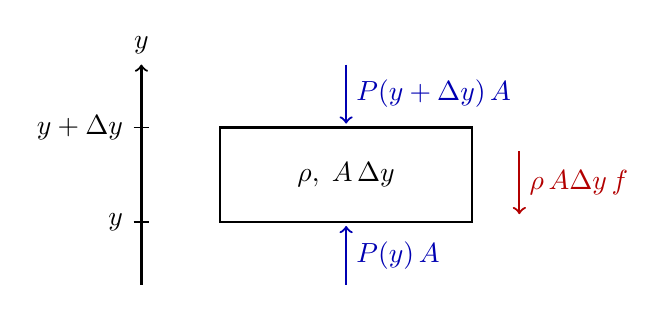
\begin{tikzpicture}[scale=1.0]
        \draw[thick] (0,0) rectangle (3.2,1.2);
        \node at (1.6,0.6) {$\rho,\;A\,\Delta y$};
        % pressures
        \draw[->,thick,blue!70!black] (1.6,-0.8) -- (1.6,-0.05)
            node[midway,right] {$P(y)\,A$};
        \draw[->,thick,blue!70!black] (1.6,2.0) -- (1.6,1.25)
            node[midway,right] {$P(y+\Delta y)\,A$};
        % gravity
        \draw[->,thick,red!70!black] (3.8,0.9) -- (3.8,0.1)
            node[midway,right] {$\rho\,A\Delta y\,f$};
        % coordinates
        \draw[thick,->] (-1.0,-0.8) -- (-1.0,2.0) node[above] {$y$};
        \draw (-1.1,0) -- (-0.9,0) node[left=6pt] {$y$};
        \draw (-1.1,1.2) -- (-0.9,1.2) node[left=6pt] {$y+\Delta y$};
    \end{tikzpicture}
    \caption{Force balance on a fluid slab of area $A$ and thickness
    $\Delta y$: the pressure below pushes up, the pressure above pushes down,
    and the external body force (per unit mass $f$, e.g.\ gravity
    $f=-g$) acts on the mass $\rho A\Delta y$.}
    \label{fig:lec09:hydrostatic-slab}
\end{figure}

\subsubsection*{Derivation}
Consider a slab of fluid of horizontal area $A$ between heights $y$ and
$y+\Delta y$, in a fluid of density $\rho$, subject to an external force per
unit mass $f$ (for gravity, $f=-g$). The net vertical force is
\begin{equation}
    F_{\rm net}
    =
    P(y)\,A-P(y+\Delta y)\,A+\rho\,A\Delta y\,f.
    \label{eq:lec09:slab-forces}
\end{equation}
Divide by the volume $A\Delta y$ and take $\Delta y\to0$:
\begin{equation}
    \frac{P(y)-P(y+\Delta y)}{\Delta y}+\rho f
    \;\xrightarrow[\Delta y\to0]{}\;
    -\dv{P}{y}+\rho f.
    \label{eq:lec09:slab-limit}
\end{equation}
In static equilibrium the net force vanishes, and in general geometry the
pressure derivative becomes a gradient:
\begin{equation}
    \boxed{
    \grad P=\rho\,\vb*{f}.
    }
    \label{eq:lec09:hydrostatic-equilibrium}
\end{equation}
\textit{Significance:} Hydrostatic equilibrium --- the pressure gradient
exactly balances the body force --- is the zeroth-order description of every
star, planet, atmosphere, and ocean.

If the element is \emph{not} in equilibrium, the net force per unit volume
accelerates it. The acceleration of a moving fluid element is the
\emph{Lagrangian (material) derivative} of the velocity:
\begin{equation}
    \dv{\vb*{v}}{t}\bigg|_{\rm following}
    \equiv
    \frac{D\vb*{v}}{Dt}
    =
    \pdv{\vb*{v}}{t}
    +\left(\vb*{v}\vdot\grad\right)\vb*{v},
    \label{eq:lec09:material-derivative}
\end{equation}
because in a time $\dd t$ the element moves to a new position where the
velocity field differs both because the field changed in time
($\partial_t\vb*{v}$) and because the element sampled a new location
($(\vb*{v}\vdot\grad)\vb*{v}$). Newton's second law per unit volume is then
the Euler equation:
\begin{equation}
    \boxed{
    \rho\left[
    \pdv{\vb*{v}}{t}
    +\left(\vb*{v}\vdot\grad\right)\vb*{v}
    \right]
    =
    -\grad P+\rho\,\vb*{f}.
    }
    \label{eq:lec09:euler-equation}
\end{equation}
\textit{Significance:} Even a flow that is steady in time
($\partial_t\vb*{v}=0$) accelerates its elements --- a drop of ink injected
into a steady stream speeds up and slows down along its streamline; the
advective term $(\vb*{v}\vdot\grad)\vb*{v}$ captures exactly this. Setting
$\vb*{v}=0$ recovers Eq.~\eqref{eq:lec09:hydrostatic-equilibrium}.

\nt{Pitfall: the material derivative is of the velocity \emph{field
evaluated along the trajectory}, not of the field at a fixed point. Forgetting
the advective term is the classic error; it is the entire difference between
$\partial\vb*{v}/\partial t$ and the acceleration a fluid element actually
feels. The full derivation is given in the continuum-mechanics course notes.}

\subsubsection*{What Holds Up a Star --- and a White Dwarf}
For an ordinary star like the Sun, the chain of causation is: gravity tries to
collapse the star $\to$ compression raises the central temperature $\to$
nuclear reactions ignite and maintain a high central temperature $\to$ the hot
center has high pressure, and the resulting $\grad P$ balances gravity
(Eq.~\eqref{eq:lec09:hydrostatic-equilibrium}). The radiated luminosity is a
by-product of maintaining this gradient.

When the fuel is exhausted the core contracts. For a star of the Sun's mass,
after helium burning produces carbon and oxygen, the core never gets hot
enough to ignite them; it contracts until a completely different pressure
source takes over --- one that requires no temperature at all. At enormous
densities the electrons are forced (Pauli exclusion) into ever higher momentum
states up to the Fermi level, and by the uncertainty principle confinement to
a smaller volume raises their momenta further. The resulting
\emph{degeneracy pressure} balances gravity: that object is a white dwarf.

\subsubsection*{Setup for the Chandrasekhar Mass (continued next lecture)}
Consider a white dwarf of mass $M$ and radius $R$, composed of nuclei with
mass number $A$ and atomic number $Z$, and define the number of electrons per
nucleon
\begin{equation}
    \beta\equiv\frac{Z}{A}.
    \label{eq:lec09:beta-definition}
\end{equation}
Then the number of nuclei and of electrons in the star are
\begin{equation}
    N_{\rm nuc}=\frac{M}{A\,m_p},
    \qquad
    N_e=Z\,N_{\rm nuc}=\beta\,\frac{M}{m_p}.
    \label{eq:lec09:electron-count}
\end{equation}
The plan, executed next week, is pure equipartition: estimate the kinetic
energy of the electrons from the Fermi level (first non-relativistically, then
relativistically) and equate it to the gravitational binding energy
$\sim GM^2/R$. The relativistic case will yield a \emph{maximal} mass --- the
Chandrasekhar mass.

\nt{Astrophysical aside from class: when the Sun becomes a red giant its
envelope will swell to roughly the present Earth--Sun distance, but the Earth
will not be engulfed: the Sun loses mass, and conservation of the Earth's
angular momentum moves its orbit outward to roughly Mars's present orbit. The
leftover core --- a white dwarf of surface temperature thousands of kelvin ---
will tidally lock the Earth, cooking one hemisphere and freezing the other.
The Moon's slightly pear-like shape is a fossil of the same tidal physics: it
solidified while still close to the Earth and froze in the tidal distortion of
that epoch.}

%%----------------------------------------------------------------------------
\subsection{Summary: The Estimation Toolbox After This Lecture}
\label{sec:lec09:summary}
%%----------------------------------------------------------------------------

\begin{enumerate}
    \item A convecting layer under everyday conditions is fully characterized
    by $(\mathrm{Ra},\mathrm{Pr})$; the auxiliary small parameters
    $\alpha\Delta T$ (linearity) and $\alpha gH/c_p$ (gravitational
    energetics) must be checked, and only enter for extreme systems.
    \item Velocities, fluxes, and any other output of the convection are a
    dimensional prefactor (built from $g\alpha\Delta T H$) times an unknown
    order-unity function of $(\mathrm{Ra},\mathrm{Pr})$ to be measured once.
    \item New physics (shear, compressibility, radiation) is admitted by
    comparing the energies or rates of the new process to the internal ones:
    Richardson number for shear, Mach number for compressibility, and the
    convective-to-radiative loss ratio for stellar envelopes.
    \item Equipartition --- equate the energy reservoirs and solve for the
    unknown --- yields the Bohr radius, anharmonic ground states, oscillator
    frequencies, ISM energy densities, and (next week) the Chandrasekhar
    mass, all up to honest order-unity factors.
\end{enumerate}
